\setcounter{subsection}{0}
\section{DISEÑO DE LA SOLUCIÓN}

Partiendo de los requerimientos de la Tabla~\ref{tab:req-resumen}, este capítulo desarrolla la Fase~2, que cubre el objetivo específico OE2. Para ello sigue las disciplinas de diseño del Proceso Unificado de Rational (RUP) y usa la norma IEEE~1016 como estructura del Documento de Diseño de Software (SDD). La arquitectura se evalúa con ATAM \citep{bass_software_2021}, un método que contrasta alternativas con escenarios de calidad (Sección~\ref{sec:alternativas}), y se describe con el modelo 4+1 \citep{kruchten_41_1995}, la notación C4 \citep{brown_c4_2018} y la norma ISO/IEC/IEEE 42010 \citep{iso_42010_2022}.

% =====================================================================
\subsection{Modelo de negocio}
\label{sec:modelo-negocio}

El diseño parte del modelo de negocio de Tukit, que la Figura~\ref{fig:canvas} resume en los
nueve bloques del lienzo de Osterwalder y Pigneur \citep{osterwalder_business_2010}.\par

\begin{figure}[!tb]
\centering
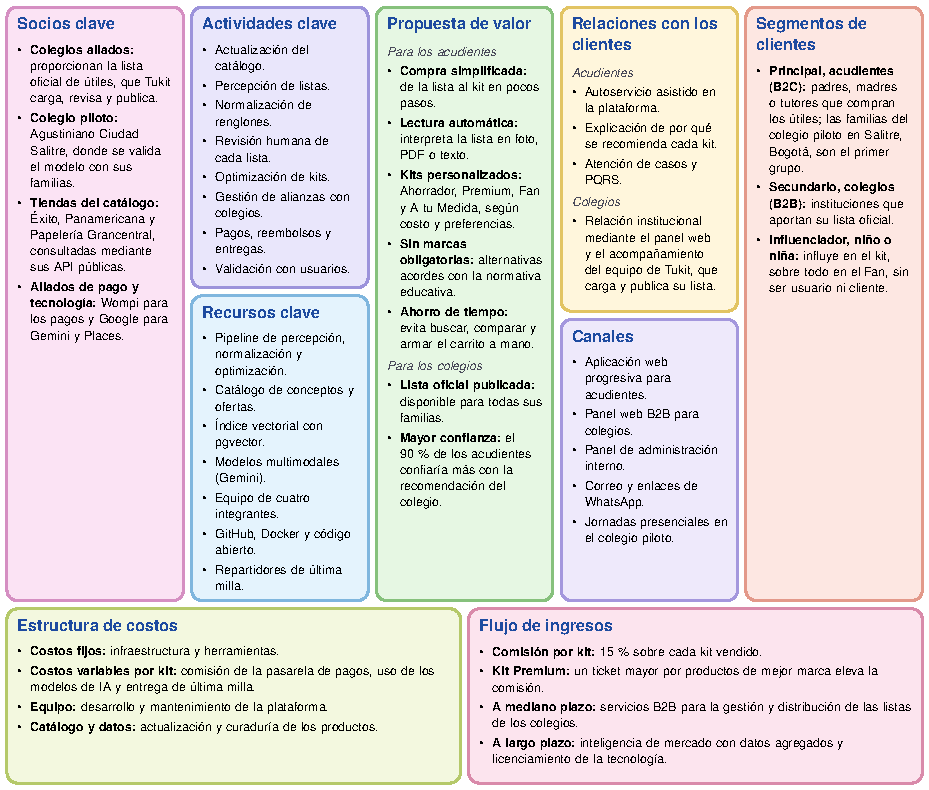
\includegraphics[width=0.42\textwidth]{negocio/canvas-modelo-negocio}
\caption{Lienzo del modelo de negocio de Tukit. Adaptado de Osterwalder y Pigneur
\citep{osterwalder_business_2010}.}
\label{fig:canvas}
\end{figure}

Varios bloques del lienzo se vuelven decisiones de arquitectura: los canales dan las dos aplicaciones, las actividades de lectura y optimización son las etapas del \emph{pipeline}, y el catálogo, los pagos y las entregas dan origen a tres servicios. Los costos e ingresos se estiman en la Sección~\ref{sec:viabilidad}.\par

% =====================================================================
\subsection{Marco de la descripción y fuerzas del diseño}
\label{sec:impulsores}

Conforme a la norma 42010, una descripción arquitectónica nombra a sus interesados, sus preocupaciones y la vista que atiende cada una. La Tabla~\ref{tab:interesados} lo hace para Tukit y la Tabla~\ref{tab:impulsores} resume los tres impulsores, las razones de diseño que deciden cómo se divide el sistema. Ninguno depende de la carga: la infraestructura mínima supera la demanda proyectada unas mil veces, así que la escalabilidad no puede ser el criterio de división.

\begin{table}[!htb]
\centering
\caption{Interesados, preocupaciones y vista que las atiende}
\label{tab:interesados}
\small
\begin{tabular}{@{}p{3.0cm}p{6.6cm}p{4.2cm}@{}}
\toprule
\textbf{Interesado} & \textbf{Preocupación} & \textbf{Vista} \\
\midrule
Acudiente & Obtener kits completos y pagar sin exponer datos de tarjeta (RNF01, RNF03) & Contexto, proceso \\
Colegio y equipo de Tukit & Revisar listas y kits; operar el sistema con cuatro personas & Contenedores, despliegue \\
Responsable de datos & Cumplir la Ley 1581 de 2012 con los datos de menores & Dominio, autorización \\
Evaluador y equipo de desarrollo & Fronteras verificables y fallas aisladas entre servicios (RNF08) & Desarrollo, decisiones \\
\bottomrule
\end{tabular}
\end{table}

\begin{table}[!htb]
\centering
\caption{Impulsores arquitectónicos de la descomposición en servicios}
\label{tab:impulsores}
\small
\begin{tabular}{@{}p{3.0cm}p{10.8cm}@{}}
\toprule
\textbf{Impulsor} & \textbf{Qué separa} \\
\midrule
Recuperabilidad asimétrica & El catálogo se reconstruye desde sus archivos de datos y admite perder hasta un día de cambios (requisito CF-02a), mientras que un pedido no admite ninguna pérdida. Compartir almacén obliga a dimensionar el respaldo por el más exigente \\
\addlinespace
Frontera de cumplimiento & La Ley 1581 \citep{congreso_ley1581_2012} y el Decreto 1377 de 2013 \citep{presidencia_decreto1377_2013} exigen consentimiento y protección reforzada de los datos de menores; aislarlos con base y llaves propias reduce lo que debe auditarse \\
\addlinespace
Perfil de recurso & La inferencia y la optimización multiobjetivo consumen CPU y memoria; la gestión transaccional exige disponibilidad y consistencia. \\
\bottomrule
\end{tabular}
\end{table}

% =====================================================================
% =====================================================================
\subsection{Descomposición en seis desplegables}
\label{sec:consolidacion}

La arquitectura pasó de catorce servicios a seis desplegables, porque catorce canales de integración son más de lo que un equipo de cuatro personas puede operar frente a decenas de pedidos diarios en temporada (el pico de diseño de RNF05 es de unos 1.000). Los tres impulsores fijaron las fronteras: los colegios pertenecen a identidad y el catálogo se separa de comercio porque sus objetivos de recuperación no permiten compartir almacén. El resultado son cinco servicios de dominio (Tabla~\ref{tab:servicios}) y la puerta de enlace, el punto único de entrada, sobre cinco bases.

Fowler \citep{fowler_monolithfirst_2015} recomienda empezar por un monolito, pero un almacén único impone el mismo objetivo de recuperación a pedidos y catálogo; por eso son seis servicios gruesos, con fronteras solo donde los datos lo exigen.


% =====================================================================
\subsection{Evaluación de la arquitectura con ATAM}
\label{sec:alternativas}

Un escenario de calidad es una situación concreta con una medida de éxito, por ejemplo optimizar un kit en menos de 8 s. Contra ellos se evaluó la arquitectura con una matriz ponderada de diez criterios. Se evaluaron tres alternativas: A, un monolito modular con almacén único; B, microservicios de grano fino, y B$'$, servicios agrupados por razón de cambio. La Tabla~\ref{tab:alternativas} los contrasta.

\begin{table}[!htb]
\centering
\caption{Alternativas arquitectónicas evaluadas}
\label{tab:alternativas}
\small
\begin{tabular}{@{}p{2.6cm}p{3.5cm}p{3.5cm}p{4.1cm}@{}}
\toprule
& \textbf{A. Monolito modular} & \textbf{B. Microservicios de grano fino} & \textbf{B$'$. Grano grueso (elegida)} \\
\midrule
Componentes & 1 desplegable, módulos internos & 13 servicios y puerta de enlace & 5 servicios de dominio y puerta de enlace, 5 bases \\
\addlinespace
Aislamiento de datos de menores & Por convención de código & Por servicio & Por servicio, base y llaves \\
\addlinespace
Punto de recuperación & Único para todo & Por servicio & Diferenciado por criticidad \\
\addlinespace
Complejidad operativa & Baja & Alta: coordinación distribuida en cada transacción & Media \\
\addlinespace
Costo de infraestructura & Mínimo & Alto & Moderado \\
\addlinespace
Puntaje ponderado (sobre 5,00) & 2,82 & 3,44 & 3,91 \\
\bottomrule
\end{tabular}
\end{table}

La alternativa~A se descarta por el primer impulsor, y la~B porque separar pedidos, inventario y pago convierte cada compra en una transacción distribuida \citep{newman_building_2021}. La~B$'$ aísla donde el cumplimiento y la recuperabilidad lo exigen.

\textbf{Sensibilidad a los pesos.} Al perturbar cada uno de los diez pesos en $\pm 20$\,\%, gana B$'$ en las veinte combinaciones (3,88 a 3,94, frente a 3,38 a 3,50 de B y 2,77 a 2,88 de A), con una ventaja mínima de 0,40 puntos sobre B.

La Tabla~\ref{tab:escenarios} contrasta cada decisión con su escenario.

\begin{table}[!htb]
\centering
\caption{Escenarios de calidad, decisión, compromiso, prueba y resultado medido}
\label{tab:escenarios}
\footnotesize
\setlength{\tabcolsep}{3pt}
\begin{tabular}{@{}p{2.4cm}p{2.7cm}p{3.0cm}p{2.9cm}p{2.9cm}@{}}
\toprule
\textbf{Escenario} & \textbf{Decisión} & \textbf{Riesgo o compromiso} & \textbf{Función de aptitud o prueba} & \textbf{Resultado medido} \\
\midrule
Optimizar un kit en menos de 8 s (escenario ESC-D4 del ATAM, rendimiento) & NSGA-II en el servicio de inteligencia, sin salto de red & El lenguaje queda fijo en Python & Prueba de latencia del escenario & p95 de 0,31 s frente a 8 s \\
\addlinespace
Carga hasta 100 usuarios (prueba de carga L-02, requisito RNF05) & Servicios independientes sobre cinco bases & El catálogo corre en un proceso y llega al 100\,\% de un núcleo & Rampa de carga en un Apple M4 & 0 errores hasta 100 usuarios; p95 del catálogo de 2,5 s con 100 \\
\addlinespace
Ráfaga de peticiones abusivas & Límite de tasa en la puerta de enlace (Redis opcional) & Si Redis cae, el conteo pasa a la memoria de la puerta & Prueba con 5 usuarios a través de la puerta & 30.257 de 31.457 peticiones respondidas con 429 \\
\addlinespace
Caída del catálogo (escenario ESC-R2, resiliencia) & Disyuntor con respaldo & Con el catálogo colgado, cada llamada agota su espera hasta que el disyuntor abre & Ensayo de degradación & El disyuntor abrió a los 26,3 s, dentro de los 30 s \\
\bottomrule
\end{tabular}
\end{table}

% =====================================================================
\subsection{Vistas de contexto, contenedores y despliegue}
\label{sec:vistas}

La vista de contexto (Figura~\ref{fig:c4-contexto}) es el nivel 1 de C4 y muestra a Tukit como un solo sistema: el acudiente y el equipo interactúan con él, y este depende de Gemini (lectura de listas y vectores), Wompi (pagos), los canales de aviso, Google Maps y las tiendas.

\begin{figure}[!htb]
\centering
\resizebox{\textwidth}{!}{% Vista de contexto (C4 nivel 1): Tukit como un solo sistema frente a sus personas y a los sistemas externos,
% agrupados por función. Estilos locales y misma paleta que c4-contenedores.tex; solo usa arrows.meta y shapes.geometric.

\definecolor{tkPerF}{HTML}{FFF0B8}\definecolor{tkPerB}{HTML}{9A7B00}
\definecolor{tkAppF}{HTML}{CFE2F7}\definecolor{tkAppB}{HTML}{1F4E86}
\definecolor{tkProcF}{HTML}{D3EDD0}\definecolor{tkProcB}{HTML}{2E6B2B}
\definecolor{tkExtF}{HTML}{FAD7B5}\definecolor{tkExtB}{HTML}{A8500F}
\definecolor{tkInfF}{HTML}{DEDEDE}\definecolor{tkInfB}{HTML}{4D4D4D}
\definecolor{tkBdF}{HTML}{CDEBEB}\definecolor{tkBdB}{HTML}{1C6E6E}
\definecolor{tkMqF}{HTML}{E2D6F4}\definecolor{tkMqB}{HTML}{5B2E99}
\begin{tikzpicture}[x=1cm, y=1cm, font=\scriptsize,
  per/.style={draw, thick, rounded corners=7pt, align=center, draw=tkPerB, fill=tkPerF, inner sep=3pt, minimum height=7mm},
  cont/.style={draw, rounded corners=2pt, align=center, draw=tkAppB, fill=tkAppF, inner sep=2pt, minimum height=8mm},
  proc/.style={draw, rounded corners=2pt, align=center, draw=tkProcB, fill=tkProcF, inner sep=2pt, minimum height=7mm},
  ext/.style={draw, rounded corners=2pt, align=center, draw=tkExtB, fill=tkExtF, inner sep=2pt, minimum height=7mm},
  infra/.style={draw, rounded corners=2pt, align=center, draw=tkInfB, fill=tkInfF, inner sep=2pt, minimum height=7mm},
  bd/.style={draw, cylinder, shape border rotate=90, aspect=0.22, align=center, fill=tkBdF,
    minimum width=1.25cm, draw=tkBdB, minimum height=8mm, inner sep=1pt},
  grupo/.style={draw=black!55, rounded corners=3pt, fill=black!4},
  http/.style={-{Stealth[length=1.6mm]}, semithick},
  evt/.style={-{Stealth[length=1.6mm]}, densely dashed, semithick},
  cola/.style={-{Stealth[length=1.6mm]}, semithick, draw=tkMqB},
  hueco/.style={draw=white, line width=2.8pt},
  paso/.style={circle, draw, fill=white, inner sep=0.5pt, font=\scriptsize\bfseries, minimum size=4.4mm},
  rot/.style={font=\scriptsize, fill=white, inner sep=1pt},
  sin/.style={semithick},
  sis/.style={draw, thick, rounded corners=3pt, align=center, draw=tkAppB, fill=tkAppF, inner sep=4pt},
  et/.style={font=\scriptsize, fill=white, inner sep=1pt, align=center, text width=3.4cm, anchor=south}]

% Flechas: etiqueta sobre la flecha, con la información que pasa
\def\fl#1#2#3#4{\draw[http] (#1,#3) -- (#2,#3) node[et, pos=0.5, yshift=-0.5pt] {#4};}
\def\fn#1#2#3#4{\draw[sin] (#1,#3) -- (#2,#3) node[et, pos=0.5, yshift=-0.5pt] {#4};}
% Sistema: un solo recuadro, como en el nivel 1 de C4
\node[sis, minimum width=3.4cm, minimum height=12.4cm, anchor=north] (tukit) at (0,1.1) {};
\node[align=center, text width=3.0cm, font=\small] at (0,-2.2) {\textbf{Tukit}\\[2pt]\scriptsize sistema de software que lee listas de útiles escolares y arma kits optimizados};
\node[align=center, text width=2.9cm, font=\scriptsize] at (0,-7.4) {aplicación web, panel de administración, puerta de enlace y cinco servicios, que se abren en la vista de contenedores};
% Personas
\node[per, text width=3.0cm] (acudiente) at (-9.6,-1.9) {\textbf{Acudiente}\\padre o madre del estudiante};
\node[per, text width=3.0cm] (equipo) at (-9.6,-6.9) {\textbf{Equipo de Tukit}\\administrador y operador de última milla};
% Sistemas externos, agrupados por función
\def\gr#1#2#3{\draw[grupo] (7.4,#1) rectangle (11.4,#2); \node[font=\scriptsize\bfseries, anchor=north] at (9.4,#1) {\vphantom{Ag}#3};}
\gr{1.1}{-1.9}{Papelerías y proveedores}
\node[ext, text width=3.4cm] at (9.4,-0.5) {\textbf{Tiendas en línea}\\Éxito, Panamericana, Librería Nacional};
\gr{-2.5}{-4.5}{Pasarela de pago}
\node[ext, text width=3.4cm] at (9.4,-3.6) {\textbf{Wompi}\\transacción y confirmación};
\gr{-5.1}{-7.1}{Lectura de listas}
\node[ext, text width=3.4cm] at (9.4,-6.2) {\textbf{Gemini}\\lectura de listas y vectores};
\gr{-7.7}{-10.5}{Canales de aviso}
\node[ext, text width=3.4cm] at (9.4,-8.9) {\textbf{Correo saliente}\\SMTP};
\node[ext, text width=3.4cm] at (9.4,-9.75) {\textbf{WhatsApp}\\enlace wa.me};
\gr{-11.1}{-13.1}{Mapas y direcciones}
\node[ext, text width=3.4cm] at (9.4,-12.2) {\textbf{OpenStreetMap}\\sugerencias de dirección};
% Acudiente
\fl{-8.1}{-1.7}{-1.1}{lista, hijos, preferencias, presupuesto, pago}
\draw[http] (-1.7,-2.5) -- (-8.1,-2.5) node[et, pos=0.5, yshift=-0.5pt] {tres kits, precios, estado del pedido};
% Equipo
\fl{-8.1}{-1.7}{-5.3}{validación de listas y mapeos, catálogo, colegios}
\draw[http] (-1.7,-6.2) -- (-8.1,-6.2) node[et, pos=0.5, yshift=-0.5pt] {cola de revisión, métricas, casos};
\fl{-8.1}{-1.7}{-7.1}{estado de la entrega, incidencias}
\draw[http] (-1.7,-8.0) -- (-8.1,-8.0) node[et, pos=0.5, yshift=-0.5pt] {pedidos por entregar, dirección, kit};
% Externos
\fl{1.7}{7.4}{-0.0}{búsqueda de productos}
\draw[http] (7.4,-0.9) -- (1.7,-0.9) node[et, pos=0.5, yshift=-0.5pt] {productos y precios};
\fl{1.7}{7.4}{-3.0}{transacción, monto, referencia}
\draw[http] (7.4,-3.9) -- (1.7,-3.9) node[et, pos=0.5, yshift=-0.5pt] {confirmación de pago};
\fl{1.7}{7.4}{-5.6}{páginas de la lista, renglones}
\draw[http] (7.4,-6.5) -- (1.7,-6.5) node[et, pos=0.5, yshift=-0.5pt] {renglones leídos, vectores};
\fl{1.7}{7.4}{-8.9}{aviso por correo}
\fn{1.7}{7.4}{-9.75}{aviso como enlace wa.me}
\fl{1.7}{7.4}{-11.6}{texto de la dirección}
\draw[http] (7.4,-12.5) -- (1.7,-12.5) node[et, pos=0.5, yshift=-0.5pt] {direcciones sugeridas};
% Leyenda
\def\tkley#1#2#3#4{\node[#1, minimum width=7mm, minimum height=4.2mm, inner sep=0pt, text width=7mm] (l#2) at #3 {};
  \node[anchor=west, font=\scriptsize, inner sep=1pt] at ([xshift=1mm]l#2.east) {#4};}
\node[draw=black!40, rounded corners=2pt, anchor=north west, minimum width=22.9cm, minimum height=1.3cm,
  inner sep=0pt] (cajaley) at (-11.4,-13.8) {};
\node[anchor=north west, font=\scriptsize\bfseries] at ([shift={(2mm,-1mm)}]cajaley.north west) {Leyenda};
\begin{scope}[shift={(cajaley.north west)}]
\tkley{per}{a}{(2.2,-0.8)}{Persona}
\tkley{sis}{b}{(4.9,-0.8)}{Sistema construido}
\tkley{ext}{d}{(8.7,-0.8)}{Sistema externo}
\draw[grupo] (11.6,-0.6) rectangle +(0.7,-0.4); \node[anchor=west, font=\scriptsize, inner sep=1pt] at (12.4,-0.8) {Agrupación por función};
\draw[http] (15.6,-0.8) -- +(0.9,0); \node[anchor=west, font=\scriptsize, inner sep=1pt] at (16.6,-0.8) {Petición, con lo que pasa};
\draw[sin] (20.0,-0.8) -- +(0.6,0); \node[anchor=west, font=\scriptsize, inner sep=1pt] at (20.7,-0.8) {Enlace};
\end{scope}
\end{tikzpicture}
}
\caption[Vista de contexto: Tukit frente a sus actores y sistemas externos.]{Vista de contexto
(C4 nivel 1): Tukit como un solo sistema frente a sus actores (el padre es el acudiente) y a los
sistemas externos, agrupados por función. Cada flecha lleva la información que pasa.}
\label{fig:c4-contexto}
\end{figure}

La vista de contenedores (Figura~\ref{fig:c4-contenedores}, C4 nivel 2) abre el sistema. Las dos aplicaciones llaman a la puerta de enlace y RabbitMQ lleva los eventos entre servicios. Las etiquetas A, B y C numeran la subida de la lista, el pago y los avisos. La de componentes (Sección~\ref{sec:vista-logica}) abre un solo servicio y la de despliegue (Sección~\ref{sec:vista-fisica}) ubica los procesos en la infraestructura.

\begin{figure}[p]
\centering
\resizebox{0.84\textwidth}{!}{% Vista de contenedores (C4 nivel 2) del código fuente del sistema en su versión del 24 de octubre de 2026,
% con los flujos de la subida y los kits (A), el pago (B) y los avisos (C). Estilos locales: no depende del
% preámbulo; solo usa las bibliotecas arrows.meta y shapes.geometric.
\definecolor{tkPerF}{HTML}{FFF0B8}\definecolor{tkPerB}{HTML}{9A7B00}
\definecolor{tkAppF}{HTML}{CFE2F7}\definecolor{tkAppB}{HTML}{1F4E86}
\definecolor{tkProcF}{HTML}{D3EDD0}\definecolor{tkProcB}{HTML}{2E6B2B}
\definecolor{tkExtF}{HTML}{FAD7B5}\definecolor{tkExtB}{HTML}{A8500F}
\definecolor{tkInfF}{HTML}{DEDEDE}\definecolor{tkInfB}{HTML}{4D4D4D}
\definecolor{tkBdF}{HTML}{CDEBEB}\definecolor{tkBdB}{HTML}{1C6E6E}
\definecolor{tkMqF}{HTML}{E2D6F4}\definecolor{tkMqB}{HTML}{5B2E99}
\begin{tikzpicture}[x=1cm, y=1cm, font=\scriptsize,
  per/.style={draw, thick, rounded corners=7pt, align=center, draw=tkPerB, fill=tkPerF, inner sep=3pt, minimum height=7mm},
  cont/.style={draw, rounded corners=2pt, align=center, draw=tkAppB, fill=tkAppF, inner sep=2pt, minimum height=8mm},
  proc/.style={draw, rounded corners=2pt, align=center, draw=tkProcB, fill=tkProcF, inner sep=2pt, minimum height=7mm},
  ext/.style={draw, rounded corners=2pt, align=center, draw=tkExtB, fill=tkExtF, inner sep=2pt, minimum height=7mm},
  infra/.style={draw, rounded corners=2pt, align=center, draw=tkInfB, fill=tkInfF, inner sep=2pt, minimum height=7mm},
  bd/.style={draw, cylinder, shape border rotate=90, aspect=0.22, align=center, fill=tkBdF,
    minimum width=1.25cm, draw=tkBdB, minimum height=8mm, inner sep=1pt},
  grupo/.style={draw=black!55, rounded corners=3pt, fill=black!4},
  http/.style={-{Stealth[length=1.6mm]}, semithick},
  evt/.style={-{Stealth[length=1.6mm]}, densely dashed, semithick},
  cola/.style={-{Stealth[length=1.6mm]}, semithick, draw=tkMqB},
  hueco/.style={draw=white, line width=2.8pt},
  paso/.style={circle, draw, fill=white, inner sep=0.5pt, font=\scriptsize\bfseries, minimum size=4.4mm},
  rot/.style={font=\scriptsize, fill=white, inner sep=1pt},
  col/.style={anchor=north west, text width=4.9cm, align=left, inner sep=0pt, font=\scriptsize}]
% Personas y aplicaciones
\node[per, text width=2.6cm] (acudiente) at (2.45,0) {\textbf{Acudiente}};
\node[per, text width=3.8cm] (equipo) at (8.6,0) {\textbf{Equipo de Tukit}\\operador y administrador};
\node[cont, text width=3.4cm] (web) at (2.45,-1.45) {\textbf{Aplicación web progresiva}\\Next.js, puerto 3000};
\node[ext, text width=1.85cm] (google_places) at (5.5,-1.45) {\textbf{Google Maps}\\sugerencias de dirección};
\node[cont, text width=3.4cm] (admin) at (8.6,-1.45) {\textbf{Panel de administración}\\Next.js, puerto 3001};
\node[ext, text width=2.5cm] (wompi) at (13.4,-1.45) {\textbf{Wompi}\\pasarela de pago};
\node[cont, minimum width=14.3cm, text width=14cm] (gateway) at (7.35,-2.85) {\textbf{Puerta de enlace}
  (Python, puerto 8010): reenvía cada petición al servicio que atiende el prefijo de su ruta};
% Servicios que llaman a otros: operación, inteligencia y comercio
\draw[grupo] (0.2,-3.65) rectangle (4.55,-6.25);
\draw[grupo] (4.85,-3.65) rectangle (10.15,-6.25);
\draw[grupo] (10.45,-3.65) rectangle (14.95,-6.25);
\node[cont, text width=2.3cm] (operacion) at (1.6,-4.3) {\textbf{Operación}\\puerto 8015};
\node[bd] (base_operacion) at (3.7,-4.3) {base de\\operación};
\node[proc, text width=1.7cm] (instantanea) at (1.2,-5.55) {instantánea de métricas (a mano)};
\node[proc, text width=1.7cm] (repartidor) at (3.5,-5.55) {repartidor de avisos};
\node[cont, text width=2.1cm] (inteligencia) at (6.4,-4.3) {\textbf{Inteligencia}\\puerto 8013};
\node[bd] (base_inteligencia) at (9.2,-4.3) {base y cola\\de trabajos};
\node[proc, text width=1.45cm] (sondeador_listas) at (5.75,-5.55) {sondeador\\de listas};
\node[proc, text width=1.45cm] (trabajador) at (7.5,-5.55) {trabajador\\durable};
\node[proc, text width=1.45cm] (publicador_inteligencia) at (9.25,-5.55) {publicador\\de eventos};
\node[cont, text width=2.4cm] (comercio) at (11.85,-4.3) {\textbf{Comercio}\\puerto 8014};
\node[bd] (base_comercio) at (13.95,-4.3) {base de\\comercio};
\node[proc, text width=1.6cm] (barredor) at (11.5,-5.55) {barredor de reservas};
\node[proc, text width=1.45cm] (publicador_comercio) at (13.75,-5.55) {publicador\\de eventos};
% Bus de llamadas a identidad y catálogo, que no llaman a otros servicios
\draw[semithick] (2.95,-6.7) -- (12.55,-6.7);
\foreach \x in {2.95,8.55,12.55}{\draw[semithick] (\x,-6.25) -- (\x,-6.7);}
\draw[semithick] (10.3,-3.25) -- (10.3,-6.7);
\node[rot, font=\tiny, align=left, anchor=south west, inner sep=0.5pt] at (10.6,-6.68) {llamadas HTTP a\\identidad y catálogo};
% RabbitMQ: intercambio de eventos entre las dos filas de servicios
\node[draw=tkMqB, fill=tkMqF, rounded corners=2pt, minimum width=10.35cm, minimum height=6.5mm,
  inner sep=0pt] (rabbitmq) at (9.125,-7.25) {};
\node[align=center, inner sep=0pt, font=\scriptsize] at (5.95,-7.25) {\textbf{RabbitMQ}\\[-1.5pt]intercambio tukit.eventos};
% Servicios proveedores
\draw[grupo] (2.9,-7.8) rectangle (6.75,-10.3);
\node[cont, text width=1.8cm] (identidad) at (3.95,-8.45) {\textbf{Identidad}\\puerto 8011};
\node[bd] (base_identidad) at (6.0,-8.45) {base de\\identidad};
\node[proc, text width=2.4cm] (sondeador_colegios) at (4.75,-9.65) {sondeador de colegios};
\draw[grupo] (9.05,-7.8) rectangle (13.1,-10.3);
\node[cont, text width=2.0cm] (catalogo) at (10.2,-8.45) {\textbf{Catálogo}\\puerto 8012};
\node[bd] (base_catalogo) at (12.3,-8.45) {base de\\catálogo};
\node[proc, text width=2.0cm, fill=tkProcF!45, densely dashed] (herramientas) at (10.2,-9.65) {herramientas de\\curaduría (a mano)};
\node[proc, text width=1.3cm] (publicador_catalogo) at (12.15,-9.65) {publicador\\de eventos};
% Sistemas externos
\node[ext, text width=1.9cm] (gemini) at (7.85,-8.45) {\textbf{Gemini}\\lectura y vectores};
\node[ext, text width=1.7cm] (tiendas) at (14.4,-9) {\textbf{Tiendas en línea}\\productos y precios};
\node[ext, text width=1.9cm] (correo) at (1.25,-8.45) {\textbf{Correo saliente}\\SMTP};
\node[ext, text width=1.9cm] (whatsapp) at (1.25,-9.55) {\textbf{WhatsApp}\\enlace wa.me};
% Fila de infraestructura
\node[infra, text width=4.6cm] (postgres) at (4.9,-11.05) {\textbf{PostgreSQL 16 con pgvector}\\un servidor con las
  cinco bases;\\cada una con su bandeja de salida};
\node[infra, text width=4.2cm, densely dotted, anchor=north] (redis) at (9.6,-10.45) {\textbf{Redis}, opcional\\caché de vectores y de lecturas\\y contador del límite de tasa\\de la puerta de enlace};
\node[infra, text width=3.3cm, densely dotted] (observabilidad) at (13.55,-11.05) {\textbf{Observabilidad opcional}\\OpenTelemetry y Jaeger};
% Personas, aplicaciones y pasarela
\draw[http] (acudiente) -- (web);
\draw[http] (equipo) -- (admin);
\draw[http] (web) -- (google_places);
\draw[http] (web.south) -- (web.south |- gateway.north);
\draw[http] (admin.south) -- (admin.south |- gateway.north);
\draw[http] ([xshift=2mm]web.north west) -- (0.88,0.65) -| node[rot, pos=0.25, above] {abre el widget de pago de Wompi} (wompi.north);
\draw[http] (wompi.south) -- (wompi.south |- gateway.north) node[rot, midway, right] {aviso firmado};
\draw[http] ([xshift=-2mm]comercio.north east) -- ++(0,0.45) -- (15.25,-3.45) |- (wompi.east);
\draw[http] (gateway.south -| operacion) -- (operacion.north);
\draw[http] (gateway.south -| inteligencia) -- (inteligencia.north);
\draw[http] (gateway.south -| comercio) -- (comercio.north);
% Llamadas entre servicios que llaman
\draw[http] ([xshift=-2mm]operacion.north east) -- ++(0,0.35) -| ([xshift=3mm]inteligencia.north west);
\draw[http] ([xshift=-3mm]inteligencia.north east) -- ++(0,0.4) -| ([xshift=3mm]comercio.north west);
% Llamadas a identidad y catálogo desde el bus; la del catálogo cruza RabbitMQ
\draw[http] (3.6,-6.7) -- (3.6,0 |- identidad.north);
\draw[hueco] (10.3,-6.9) -- (10.3,-7.6);
\draw[http] (10.3,-6.7) -- (10.3,0 |- catalogo.north);
% Bandejas de salida que lee cada publicador
\draw[evt] (base_inteligencia.south) -- (base_inteligencia.south |- publicador_inteligencia.north);
\draw[evt] (base_comercio.south) -- (base_comercio.south |- publicador_comercio.north);
\draw[evt] (base_catalogo.south) -- (base_catalogo.south |- publicador_catalogo.north);
% Eventos por RabbitMQ: de los publicadores al intercambio y del intercambio a la cola de cada consumidor
\foreach \x in {4.1,5.75,7.1,9.25}{\draw[hueco] (\x,-6.58) -- (\x,-6.82);}
\draw[cola] (publicador_inteligencia.south) -- (9.25,0 |- rabbitmq.north);
\draw[cola] (publicador_comercio.south) -- (13.75,0 |- rabbitmq.north);
\draw[cola] (11.5,0 |- publicador_catalogo.north) -- (11.5,0 |- rabbitmq.south);
\draw[cola] (4.1,0 |- rabbitmq.north) -- (4.1,0 |- repartidor.south);
\draw[cola] (5.75,0 |- rabbitmq.north) -- (sondeador_listas.south);
\draw[cola] (7.1,0 |- rabbitmq.north) -- (7.1,0 |- trabajador.south);
\draw[cola] (5.2,0 |- rabbitmq.south) -- (5.2,0 |- sondeador_colegios.north);
% Llamadas a sistemas externos
\draw[hueco] (7.85,-6.58) -- (7.85,-6.82);
\draw[hueco] (7.85,-6.9) -- (7.85,-7.6);
\draw[http] (7.85,0 |- trabajador.south) -- (gemini.north);
\draw[http] (catalogo.west) -- (gemini.east);
\draw[http] (13.1,-9) -- (tiendas.west);
\draw[http] (2.75,0 |- repartidor.south) |- (correo.east);
\draw[semithick] (2.75,0 |- repartidor.south) |- (whatsapp.east);
% Pasos de los flujos
\node[paso] at (2.15,-2.15) {A1};
\node[paso] at (7.85,-7.73) {A1};
\node[paso] at (10.3,-6.05) {A2};
\node[paso] at (8.3,-2.15) {A3};
\node[paso] at (5.75,-6.45) {A4};
\node[paso] at (2.75,-2.15) {B1};
\node[paso] at (11.6,0.65) {B2};
\node[paso] at (13.05,-2.15) {B3};
\node[paso] at (barredor.north west) {B4};
\node[paso] at (4.1,-6.45) {C1};
\node[paso] at (2.95,-6.45) {C2};
\node[paso] at (2.75,-9) {C3};
% Pasos de los flujos y notación, debajo de la figura
\node[col] (colA) at (0.2,-12.1) {\textbf{A. Subida de la lista y kits}\\[1pt]
  \textbf{A1} El acudiente sube la lista; inteligencia la lee con Gemini, guarda el trabajo y lo anuncia en su bandeja de salida.\\[1pt]
  \textbf{A2} Con la subida aceptada (202), el trabajador toma el trabajo de RabbitMQ o de su tabla, pide candidatos al catálogo y deja los kits por revisar.\\[1pt]
  \textbf{A3} El equipo revisa los kits en el panel y los publica; inteligencia deja el evento de kits publicados en su bandeja de salida.\\[1pt]
  \textbf{A4} Si la lista no estaba verificada, el sondeador de listas arma el kit al recibir el evento de lista verificada.};
\node[col] (colB) at (5.35,-12.1) {\textbf{B. Pago}\\[1pt]
  \textbf{B1} El acudiente elige un kit y escribe la dirección con sugerencias de Google Maps; inteligencia crea la orden en comercio, que reserva el inventario al precio vigente.\\[1pt]
  \textbf{B2} La aplicación web abre el widget de Wompi y el acudiente paga.\\[1pt]
  \textbf{B3} Wompi envía el aviso firmado o la página de resultado pide sincronizar el pago; comercio deja el evento de pedido pagado en su bandeja.\\[1pt]
  \textbf{B4} El barredor libera la reserva del pedido que no se paga en 24 horas y lo cancela.};
\node[col] (colC) at (10.5,-12.1) {\textbf{C. Avisos}\\[1pt]
  \textbf{C1} El repartidor de avisos recibe por RabbitMQ los eventos de kits publicados, pago, incidencia, despacho, reparto y entrega, y no repite el aviso de un evento ya enviado.\\[1pt]
  \textbf{C2} Pide a identidad el contacto del acudiente, sin guardarlo.\\[1pt]
  \textbf{C3} Si el acudiente tiene celular, arma un enlace de WhatsApp con el aviso; si no, se lo envía por correo.\\[1pt]
  El despacho lo registra el equipo en el panel, con el nombre y el celular del repartidor propio; las transportadoras con guía son una evolución prevista.};
\node[anchor=north west, text width=15.1cm, align=left, inner sep=0pt, font=\scriptsize]
  at ([yshift=-2mm]colA.south west |- current bounding box.south) {Línea continua: llamada HTTP. Línea discontinua:
  el publicador lee la bandeja de salida de su base. Línea violeta: evento que viaja por RabbitMQ hasta la cola de su
  consumidor (avisos, colegios, listas y trabajos), con reintentos y descartados; sin RabbitMQ, los publicadores no
  arrancan y cada consumidor lee la bandeja del productor. Línea punteada: componente opcional. Línea sin punta: enlace que el sistema
  arma y no envía. Recuadro gris: el servicio con sus procesos y su base.};
% Leyenda
\def\tkley#1#2#3#4{\node[#1, minimum width=7mm, minimum height=4.2mm, inner sep=0pt, text width=7mm] (l#2) at #3 {};
  \node[anchor=west, font=\scriptsize, inner sep=1pt] at ([xshift=1mm]l#2.east) {#4};}
\node[draw=black!40, rounded corners=2pt, anchor=north west, minimum width=15.05cm, minimum height=2.3cm,
  inner sep=0pt] (cajaley) at ([yshift=-1mm]colA.south west |- current bounding box.south) {};
\node[anchor=north west, font=\scriptsize\bfseries] at ([shift={(2mm,-1mm)}]cajaley.north west) {Leyenda};
\begin{scope}[shift={(cajaley.north west)}]
\tkley{per}{a}{(1.2,-0.75)}{Persona}
\tkley{cont}{b}{(3.9,-0.75)}{Aplicación o servicio}
\tkley{proc}{c}{(7.8,-0.75)}{Proceso en segundo plano}
\tkley{ext}{d}{(12.3,-0.75)}{Sistema externo}
\tkley{bd}{e}{(1.2,-1.35)}{Base de datos}
\tkley{infra}{f}{(3.9,-1.35)}{Infraestructura}
\node[draw=tkMqB, fill=tkMqF, rounded corners=2pt, minimum width=7mm, minimum height=4.2mm, inner sep=0pt] (lg) at (7.8,-1.35) {};
\node[anchor=west, font=\scriptsize, inner sep=1pt] at ([xshift=1mm]lg.east) {RabbitMQ};
\draw[http] (0.8,-1.95) -- +(0.9,0); \node[anchor=west, font=\scriptsize, inner sep=1pt] at (1.8,-1.95) {HTTP};
\draw[evt] (3.9,-1.95) -- +(0.9,0); \node[anchor=west, font=\scriptsize, inner sep=1pt] at (4.9,-1.95) {Evento de la bandeja};
\draw[cola] (8.4,-1.95) -- +(0.9,0); \node[anchor=west, font=\scriptsize, inner sep=1pt] at (9.4,-1.95) {Cola de RabbitMQ};
\end{scope}
\end{tikzpicture}
}
\caption{Vista de contenedores (C4 nivel 2) del sistema construido, con los procesos en
segundo plano de cada servicio y los pasos de la subida de la lista y los kits (A), el pago (B)
y los avisos (C).}
\label{fig:c4-contenedores}
\end{figure}

Cada servicio registra el evento en su bandeja de salida, en la misma operación que el cambio, y de ahí pasa a RabbitMQ en una cola por consumidor con reintentos; la entrega es al menos una vez, con consumidores idempotentes. Redis es opcional y guarda solo lo recalculable; si no responde en 250~ms, cada servicio calcula sin caché.

% =====================================================================
\subsection{Vista lógica}
\label{sec:vista-logica}

La división en componentes sigue el diseño guiado por el dominio \citep{evans_domain-driven_2004}: cada servicio es una parte del negocio con su vocabulario y sus datos. La Tabla~\ref{tab:servicios} resume cada componente, y la Figura~\ref{fig:c4-componentes} abre el servicio de inteligencia, el que concentra la lógica de lectura y optimización.

\begin{table}[!htb]
\centering\footnotesize
\setlength{\tabcolsep}{4pt}
\renewcommand{\arraystretch}{1.15}
\caption{Componentes del sistema y su responsabilidad.}
\label{tab:servicios}
\begin{tabularx}{\textwidth}{@{}p{2.9cm}X@{}}
\toprule
\textbf{Componente} & \textbf{Responsabilidad} \\
\midrule
web & El acudiente carga la lista, revisa los kits, paga, sigue pedidos y casos, y gestiona sus datos. \\
admin & El equipo revisa listas, gestiona el catálogo, consulta pedidos y entregas, y responde casos. \\
Puerta de enlace & Recibe las peticiones externas, limita su número y las dirige al servicio de su ruta. \\
Identidad & Cuentas, roles, colegios, hijos, consentimiento y supresión de datos; frontera de protección de datos personales. \\
Catálogo & Conceptos, productos, ofertas por tienda y listas oficiales; empareja cada renglón con su concepto. \\
Inteligencia & Lee, normaliza y optimiza cada lista; genera los kits y las propuestas del asistente. \\
Comercio & Pedidos, reserva de inventario, pagos, entrega y retracto. \\
Operación & Casos de soporte, notificaciones y registro de auditoría. \\
\bottomrule
\end{tabularx}
\end{table}

\begin{figure}[!htb]
\centering
\resizebox{0.9\textwidth}{!}{% Vista de componentes (C4 nivel 3) del servicio de inteligencia. Estilos locales con nombres propios;
% usa las bibliotecas arrows.meta y shapes.geometric. Misma paleta que la vista de contenedores.
\definecolor{tcCompF}{HTML}{CFE2F7}\definecolor{tcCompB}{HTML}{1F4E86}
\definecolor{tcProcF}{HTML}{D3EDD0}\definecolor{tcProcB}{HTML}{2E6B2B}
\definecolor{tcExtF}{HTML}{FAD7B5}\definecolor{tcExtB}{HTML}{A8500F}
\definecolor{tcInfF}{HTML}{DEDEDE}\definecolor{tcInfB}{HTML}{4D4D4D}
\definecolor{tcBdF}{HTML}{CDEBEB}\definecolor{tcBdB}{HTML}{1C6E6E}
\definecolor{tcMqF}{HTML}{E2D6F4}\definecolor{tcMqB}{HTML}{5B2E99}
\begin{tikzpicture}[x=1cm, y=1cm, font=\scriptsize,
  tcc/.style={draw=tcCompB, fill=tcCompF, rounded corners=2pt, align=center, inner sep=2pt, minimum height=11mm, text width=2.4cm},
  tcp/.style={draw=tcProcB, fill=tcProcF, rounded corners=2pt, align=center, inner sep=2pt, minimum height=11mm},
  tce/.style={draw=tcExtB, fill=tcExtF, rounded corners=2pt, align=center, inner sep=2pt, minimum height=9mm},
  tci/.style={draw=tcInfB, fill=tcInfF, rounded corners=2pt, align=center, inner sep=2pt, minimum height=9mm},
  tcb/.style={draw=tcBdB, fill=tcBdF, rounded corners=2pt, align=center, inner sep=2pt, minimum height=9mm},
  tcm/.style={draw=tcMqB, fill=tcMqF, rounded corners=2pt, align=center, inner sep=2pt, minimum height=9mm},
  tcf/.style={-{Stealth[length=1.6mm]}, semithick},
  tcg/.style={-{Stealth[length=1.6mm]}, semithick, densely dotted},
  tcr/.style={font=\tiny, fill=white, inner sep=1pt}]
\draw[draw=black!55, rounded corners=3pt, fill=black!4] (-0.1,0.5) rectangle (14.2,-5.7);
\node[anchor=north west, font=\scriptsize\bfseries] at (0.05,0.45) {Servicio de inteligencia (puerto 8013)};
\node[tcc, minimum width=13.2cm, text width=12.8cm] (api) at (7.05,-0.75) {\textbf{Rutas HTTP}: listas, trabajos, revisión, asistente y métricas};
\node[tcc] (per) at (1.6,-2.85) {\textbf{Percepción}\\lee cada página del PDF y decide si es la lista de un grado};
\node[tcc] (nor) at (5.0,-2.85) {\textbf{Normalización}\\separa cantidad, empaque y renglones que no se compran};
\node[tcc] (res) at (8.4,-2.85) {\textbf{Resolución}\\candidatos del catálogo y estado de cada renglón};
\node[tcc] (opt) at (11.9,-2.85) {\textbf{Optimizador}\\NSGA-II sobre los candidatos y los pesos del hogar};
\node[tcc, text width=3.4cm] (nl) at (4.6,-4.65) {\textbf{Asistente NL2C}\\convierte lo que escribe el acudiente en cambios al kit};
\node[tcc, text width=3.4cm] (trab) at (11.0,-4.65) {\textbf{Trabajos y cola de revisión}\\estado durable, trabajador, sondeador y publicador};
\node[tci, minimum width=1.3cm, densely dotted] (red) at (0.7,-7.3) {\textbf{Redis}\\caché};
\node[tce, minimum width=2.0cm] (gem) at (2.9,-7.3) {\textbf{Gemini}\\lectura};
\node[tce, minimum width=2.0cm] (cat) at (8.4,-7.3) {\textbf{Catálogo}\\emparejamiento};
\node[tcm, minimum width=1.7cm] (mq) at (10.4,-7.3) {\textbf{RabbitMQ}\\eventos};
\node[tcb, minimum width=1.7cm] (pg) at (12.6,-7.3) {\textbf{PostgreSQL}\\base propia};
% Dentro del servicio
\draw[tcf] (per) -- (nor);
\draw[tcf] (nor) -- (res);
\draw[tcf] (res) -- (opt);
\draw[tcf] (3.3,-1.3) -- (nl.north -| 3.3,0);
\draw[tcf] (13.65,-1.3) |- (trab.east -| 12.7,0);
\draw[tcf] (9.4,0 |- trab.north) -- (9.4,0 |- res.south);
\draw[tcf] (11.9,0 |- trab.north) -- node[tcr, right] {orquesta} (opt.south);
% Hacia afuera
\draw[tcg] (0.7,0 |- per.south) -- (red.north);
\draw[tcf] (2.3,0 |- per.south) -- (2.3,0 |- gem.north);
\draw[tcf] (3.9,0 |- nl.south) -- (3.9,-6.3) -- (3.5,-6.3) -- (3.5,0 |- gem.north);
\draw[tcf] (res.south) -- node[tcr, right] {HTTP} (cat.north);
\draw[tcf] (10.4,0 |- trab.south) -- (mq.north);
\draw[tcf] (12.6,0 |- trab.south) -- (pg.north);
\end{tikzpicture}
}
\caption{Vista de componentes (C4 nivel 3) del servicio de inteligencia: las etapas de percepción,
normalización, resolución y optimización, el asistente NL2C y los trabajos con su cola de revisión,
con sus dependencias externas. Línea punteada: dependencia opcional. Misma paleta que la
Figura~\ref{fig:c4-contenedores}.}
\label{fig:c4-componentes}
\end{figure}

Los datos de menores se concentran en identidad, y crear el pedido, reservar el inventario y registrar el pago ocurren en comercio, en una sola transacción. Los servicios se hablan de forma directa cuando necesitan respuesta inmediata y por eventos cuando informan un hecho, como un pago confirmado. Nunca se almacenan datos de tarjeta.

% =====================================================================
\subsection{Vista física}
\label{sec:vista-fisica}

En la vista física (Figura~\ref{fig:despliegue}) todo corre en un portátil del equipo, sin Kubernetes ni autoescalado. Docker Compose levanta PostgreSQL 16 con pgvector (las cinco bases), RabbitMQ, Redis y Jaeger, y el resto corre como procesos locales. Un túnel de Cloudflare expone la web solo durante las sesiones con acudientes, y Wompi funciona en modo simulado.

\begin{figure}[!htb]
\centering
\resizebox{0.6\textwidth}{!}{% Vista de despliegue: cómo corre Tukit en el portátil del equipo (make arriba / reanudar / backend),
% con el túnel de Cloudflare de las sesiones con acudientes. Misma paleta que c4-contenedores.tex.
\definecolor{tkPerF}{HTML}{FFF0B8}\definecolor{tkPerB}{HTML}{9A7B00}
\definecolor{tkAppF}{HTML}{CFE2F7}\definecolor{tkAppB}{HTML}{1F4E86}
\definecolor{tkProcF}{HTML}{D3EDD0}\definecolor{tkProcB}{HTML}{2E6B2B}
\definecolor{tkExtF}{HTML}{FAD7B5}\definecolor{tkExtB}{HTML}{A8500F}
\definecolor{tkInfF}{HTML}{DEDEDE}\definecolor{tkInfB}{HTML}{4D4D4D}
\definecolor{tkBdF}{HTML}{CDEBEB}\definecolor{tkBdB}{HTML}{1C6E6E}
\definecolor{tkMqF}{HTML}{E2D6F4}\definecolor{tkMqB}{HTML}{5B2E99}
\begin{tikzpicture}[x=1cm, y=1cm, font=\scriptsize,
  per/.style={draw=tkPerB, thick, rounded corners=7pt, align=center, fill=tkPerF, inner sep=3pt, minimum height=7mm},
  cont/.style={draw=tkAppB, rounded corners=2pt, align=center, fill=tkAppF, inner sep=2pt, minimum height=8mm},
  proc/.style={draw=tkProcB, rounded corners=2pt, align=center, fill=tkProcF, inner sep=2pt, minimum height=7mm},
  ext/.style={draw=tkExtB, rounded corners=2pt, align=center, fill=tkExtF, inner sep=2pt, minimum height=7mm},
  infra/.style={draw=tkInfB, rounded corners=2pt, align=center, fill=tkInfF, inner sep=2pt, minimum height=7mm},
  bd/.style={draw=tkBdB, cylinder, shape border rotate=90, aspect=0.22, align=center, fill=tkBdF, inner sep=2pt},
  mq/.style={draw=tkMqB, rounded corners=2pt, align=center, fill=tkMqF, inner sep=2pt, minimum height=7mm},
  nodo/.style={draw=black!55, rounded corners=3pt, fill=black!4},
  http/.style={-{Stealth[length=1.6mm]}, semithick},
  rot/.style={font=\tiny, fill=white, inner sep=1pt}]
% Visitante
\node[per, text width=3.2cm] (acudiente) at (1.8,0) {\textbf{Acudiente}\\navegador del celular};
\node[ext, text width=3.2cm] (tunel) at (1.8,-1.7) {\textbf{Túnel de Cloudflare}\\URL temporal, solo en las sesiones};
% Portátil
\draw[nodo] (3.9,0.6) rectangle (15.1,-9.1);
\node[anchor=north west, font=\scriptsize\bfseries] at (4.0,0.5) {Portátil del equipo (127.0.0.1)};
\node[cont, text width=3.0cm] (web) at (5.6,-1.0) {\textbf{Aplicación web}\\Next.js, puerto 3000};
\node[cont, text width=3.0cm] (admin) at (9.0,-1.0) {\textbf{Panel de administración}\\Next.js, puerto 3001};
\node[cont, text width=10.4cm] (gateway) at (9.4,-2.5) {\textbf{Puerta de enlace}, puerto 8010};
\node[cont, text width=1.6cm] (s1) at (5.0,-4.0) {\textbf{Identidad}\\8011};
\node[cont, text width=1.6cm] (s2) at (7.0,-4.0) {\textbf{Catálogo}\\8012};
\node[cont, text width=1.6cm] (s3) at (9.0,-4.0) {\textbf{Inteligencia}\\8013};
\node[cont, text width=1.6cm] (s4) at (11.0,-4.0) {\textbf{Comercio}\\8014};
\node[cont, text width=1.6cm] (s5) at (13.0,-4.0) {\textbf{Operación}\\8015};
\node[proc, text width=10.4cm] (fondo) at (9.4,-5.3) {Procesos en segundo plano de cada servicio (trabajador, publicadores, sondeadores, barredor, repartidor)};
\node[infra, text width=3.4cm] (pg) at (5.9,-7.0) {\textbf{PostgreSQL 16 con pgvector}\\5 bases, puerto 5432};
\node[mq, text width=2.8cm] (mq) at (9.4,-7.0) {\textbf{RabbitMQ}\\AMQP 5672, consola 15672};
\node[infra, text width=2.3cm, densely dotted] (redis) at (12.1,-7.0) {\textbf{Redis}\\opcional};
\node[infra, text width=1.9cm, densely dotted] (jaeger) at (14.1,-7.0) {\textbf{Jaeger}\\opcional};
\node[anchor=north west, text width=10.9cm, align=left, font=\scriptsize, inner sep=0pt] at (4.2,-7.9)
  {Un comando levanta los procesos, otro los vuelve a levantar tras un apagado y un tercero migra, siembra y levanta de cero.};
% Servicios externos
\node[ext, text width=3.2cm] (wompi) at (1.8,-4.4) {\textbf{Wompi}\\modo simulado; no sale a la red};
\node[ext, text width=3.2cm] (gemini) at (1.8,-6.5) {\textbf{Gemini}\\lectura de listas y vectores};
\node[ext, text width=3.2cm] (otros) at (1.8,-8.3) {\textbf{OpenStreetMap, correo y tiendas}\\llamadas salientes};
% Flechas
\draw[http] (acudiente) -- (tunel);
\draw[http] (tunel.east) -- ++(0.3,0) |- (web.west);
\draw[http] (web.east) -- (admin.west);
\draw[http] (web.south) -- ++(0,-0.35) -| ([xshift=-3.5cm]gateway.north);
\draw[http] (admin.south) -- (admin.south |- gateway.north);
\foreach \s in {s1,s2,s3,s4,s5}{\draw[http] (\s.north |- gateway.south) -- (\s.north);}
\draw[http] (s3.south) -- (s3.south |- fondo.north);
\draw[http] (fondo.south) -- (fondo.south |- mq.north);
\draw[http] (fondo.south -| pg.north) -- (pg.north);
\draw[http, dashed] (s3.west) -- ++(-2.7,0) |- (gemini.east);
\draw[http, dashed, densely dotted] (wompi.east) -- ++(0.2,0) |- (s4.west);
\end{tikzpicture}
}
\caption[Vista de despliegue: cómo corre Tukit en el equipo.]{Vista de despliegue. Todo el
sistema corre en un portátil, con un túnel de Cloudflare hacia la web en las sesiones con acudientes.
Misma paleta que la Figura~\ref{fig:c4-contenedores}.}
\label{fig:despliegue}
\end{figure}

% =====================================================================
\subsection{Vista de tiempo de ejecución}
\label{sec:proceso}
\label{sec:vista-procesos}

La vista de tiempo de ejecución describe cómo colaboran los componentes en las tres interacciones centrales: cargar la lista, revisarla y pagar el kit.

\paragraph{Proceso 1: cargar la lista y generar los kits.} El acudiente elige la lista oficial de su colegio y grado, o carga la suya, e indica sus preferencias. La puerta de enlace aplica el límite de tasa y reenvía a inteligencia, que registra un trabajo y responde 202 sin esperar el resultado. El trabajador durable lo toma de RabbitMQ o, si el broker no está, de la tabla; lee la lista con Gemini, normaliza cada renglón y pide candidatos al catálogo. Sin candidatos, el renglón queda como hueco; con ellos, el umbral $\tau = 0{,}75$ separa el resuelto del ambiguo. El optimizador arma los kits con NSGA-II (Figura~\ref{fig:sec-pipeline}).

\begin{figure}[!htb]
\centering
\resizebox{0.78\textwidth}{!}{% Secuencia del pipeline: lectura en la subida, trabajo asíncrono por cola, resolución y optimización. Misma paleta que c4-contenedores.tex.
\definecolor{tkPerF}{HTML}{FFF0B8}\definecolor{tkPerB}{HTML}{9A7B00}
\definecolor{tkAppF}{HTML}{CFE2F7}\definecolor{tkAppB}{HTML}{1F4E86}
\definecolor{tkProcF}{HTML}{D3EDD0}\definecolor{tkProcB}{HTML}{2E6B2B}
\definecolor{tkExtF}{HTML}{FAD7B5}\definecolor{tkExtB}{HTML}{A8500F}
\definecolor{tkInfF}{HTML}{DEDEDE}\definecolor{tkInfB}{HTML}{4D4D4D}
\definecolor{tkBdF}{HTML}{CDEBEB}\definecolor{tkBdB}{HTML}{1C6E6E}
\definecolor{tkMqF}{HTML}{E2D6F4}\definecolor{tkMqB}{HTML}{5B2E99}
\begin{tikzpicture}[x=1cm, y=1cm, font=\small,
  pa/.style={draw=tkAppB, fill=tkAppF, rounded corners=2pt, align=center, minimum width=1.95cm, minimum height=9mm},
  pg/.style={draw=tkInfB, fill=tkInfF, rounded corners=2pt, align=center, minimum width=1.95cm, minimum height=9mm},
  pp/.style={draw=tkProcB, fill=tkProcF, rounded corners=2pt, align=center, minimum width=1.95cm, minimum height=9mm},
  pc/.style={draw=tkBdB, fill=tkBdF, rounded corners=2pt, align=center, minimum width=1.95cm, minimum height=9mm},
  pr/.style={draw=tkPerB, fill=tkPerF, rounded corners=2pt, align=center, minimum width=1.95cm, minimum height=9mm},
  pe/.style={draw=tkExtB, fill=tkExtF, rounded corners=2pt, align=center, minimum width=1.95cm, minimum height=9mm},
  pm/.style={draw=tkMqB, fill=tkMqF, rounded corners=2pt, align=center, minimum width=1.95cm, minimum height=9mm},
  life/.style={dashed, draw=tkInfB!70},
  msg/.style={-{Stealth[length=1.8mm]}, thick, draw=tkAppB},
  ret/.style={-{Stealth[length=1.8mm]}, thick, dashed, draw=tkInfB},
  lab/.style={fill=white, inner sep=1pt, align=center}]
\node[pa] (w) at (0,0) {Acudiente\\(web)};
\node[pg] (g) at (2.2,0) {Puerta de\\enlace};
\node[pp] (i) at (4.4,0) {Inteli-\\gencia};
\node[pe] (m) at (6.6,0) {Gemini};
\node[pm] (q) at (8.8,0) {Cola y\\trabajador};
\node[pc] (c) at (11.0,0) {Catálogo};
\node[pr] (r) at (13.2,0) {Revisión\\humana};
\foreach \n in {w,g,i,m,q,c,r} \draw[life] (\n.south) -- ++(0,-10.7);
\draw[msg] (0,-1.1) -- (2.2,-1.1) node[midway, above=1pt, lab] {1 sube};
\draw[msg] (2.2,-1.8) -- (4.4,-1.8) node[midway, above=1pt, lab] {2 límite 429};
\draw[msg] (4.4,-2.5) -- (6.6,-2.5) node[midway, above=1pt, lab] {3 lee páginas};
\draw[ret] (6.6,-3.1) -- (4.4,-3.1) node[midway, above=1pt, lab] {4 renglones};
\draw[msg] (4.4,-3.8) -- (8.8,-3.8) node[midway, above=1pt, lab] {5 guarda el trabajo y lo encola};
\draw[ret] (4.4,-4.5) -- (0,-4.5) node[pos=0.5, above=1pt, lab] {6 responde 202: trabajo aceptado};
\draw[msg] (8.8,-5.3) -- ++(0.8,0) -- ++(0,-0.55) -- ++(-0.8,0);
\node[anchor=west, lab, align=left] at (9.7,-5.55) {7 toma el trabajo\\(RabbitMQ o tabla)};
\draw[msg] (8.8,-6.5) -- (11.0,-6.5) node[midway, above=1pt, lab] {8 pide candidatos};
\draw[ret] (11.0,-7.1) -- (8.8,-7.1) node[midway, above=1pt, lab] {9 candidatos};
\draw[msg] (8.8,-7.8) -- ++(0.8,0) -- ++(0,-1.0) -- ++(-0.8,0);
\node[anchor=west, lab, align=left] at (9.7,-8.3) {10 clasifica: sin candidatos, hueco;\\parecido $\geq \tau = 0{,}75$, resuelto;\\si no, ambiguo};
\draw[msg] (8.8,-9.4) -- ++(0.8,0) -- ++(0,-0.55) -- ++(-0.8,0);
\node[anchor=west, lab, align=left] at (9.7,-9.65) {11 NSGA-II sobre los renglones\\con candidatos};
\draw[msg] (8.8,-10.6) -- (13.2,-10.6) node[midway, above=1pt, lab] {12 kits por revisar};
\end{tikzpicture}
}
\caption{Secuencia de la subida de una lista, el trabajo asíncrono por cola, la clasificación de cada renglón y la construcción de los kits.}
\label{fig:sec-pipeline}
\end{figure}

\paragraph{Proceso 2: revisar la lista.} Cuando una lista nueva termina de procesarse, queda en la cola de revisión del administrador de Tukit. Este compara la lectura con el documento original, corrige los renglones dudosos y marca los productos no disponibles. Solo entonces los kits se publican, y la lista revisada queda disponible para las demás familias del mismo colegio y grado.


\paragraph{Proceso 3: confirmar y pagar el kit.} Al confirmar, inteligencia llama a comercio, que crea la orden de forma idempotente, verifica el precio con el catálogo y reserva el inventario. El pago no depende del regreso del acudiente: Wompi avisa por webhook (una llamada a comercio al terminar el pago), comercio verifica la firma, aplica el pago una sola vez y escribe el evento en su bandeja de salida; de ahí pasa a RabbitMQ y operación avisa al acudiente (Figura~\ref{fig:sec-pago}).

\begin{figure}[!htb]
\centering
\resizebox{0.78\textwidth}{!}{% Secuencia del pago: inteligencia crea la orden en comercio; aviso de Wompi y evento por la bandeja de salida. Misma paleta que c4-contenedores.tex.
\definecolor{tkAppF}{HTML}{CFE2F7}\definecolor{tkAppB}{HTML}{1F4E86}
\definecolor{tkProcF}{HTML}{D3EDD0}\definecolor{tkProcB}{HTML}{2E6B2B}
\definecolor{tkExtF}{HTML}{FAD7B5}\definecolor{tkExtB}{HTML}{A8500F}
\definecolor{tkInfF}{HTML}{DEDEDE}\definecolor{tkInfB}{HTML}{4D4D4D}
\definecolor{tkMqF}{HTML}{E2D6F4}\definecolor{tkMqB}{HTML}{5B2E99}
\begin{tikzpicture}[x=1cm, y=1cm, font=\small,
  pa/.style={draw=tkAppB, fill=tkAppF, rounded corners=2pt, align=center, minimum width=1.95cm, minimum height=9mm},
  pg/.style={draw=tkInfB, fill=tkInfF, rounded corners=2pt, align=center, minimum width=1.95cm, minimum height=9mm},
  pp/.style={draw=tkProcB, fill=tkProcF, rounded corners=2pt, align=center, minimum width=1.95cm, minimum height=9mm},
  pe/.style={draw=tkExtB, fill=tkExtF, rounded corners=2pt, align=center, minimum width=1.95cm, minimum height=9mm},
  pm/.style={draw=tkMqB, fill=tkMqF, rounded corners=2pt, align=center, minimum width=1.95cm, minimum height=9mm},
  life/.style={dashed, draw=tkInfB!70},
  msg/.style={-{Stealth[length=1.8mm]}, thick, draw=tkAppB},
  ret/.style={-{Stealth[length=1.8mm]}, thick, dashed, draw=tkInfB},
  lab/.style={fill=white, inner sep=1pt, align=center}]
\node[pa] (w) at (0,0) {Acudiente\\(web)};
\node[pg] (g) at (2.2,0) {Puerta de\\enlace};
\node[pp] (i) at (4.4,0) {Inteli-\\gencia};
\node[pp] (c) at (6.6,0) {Comercio};
\node[pe] (p) at (8.8,0) {Wompi};
\node[pm] (q) at (11.0,0) {RabbitMQ};
\node[pp] (o) at (13.2,0) {Operación};
\foreach \n in {w,g,i,c,p,q,o} \draw[life] (\n.south) -- ++(0,-9.8);
\draw[msg] (0,-1.1) -- (2.2,-1.1) node[midway, above=1pt, lab] {1 paga el kit};
\draw[msg] (2.2,-1.8) -- (4.4,-1.8) node[midway, above=1pt, lab] {2 reenvía};
\draw[msg] (4.4,-2.5) -- (6.6,-2.5) node[midway, above=1pt, lab] {3 crea la orden};
\draw[msg] (6.6,-3.2) -- ++(0.8,0) -- ++(0,-0.9) -- ++(-0.8,0);
\node[anchor=west, lab, align=left] at (7.5,-3.65) {4 orden idempotente; relee el precio\\y rechaza si cambió};
\draw[msg] (4.4,-4.8) -- (6.6,-4.8) node[midway, above=1pt, lab] {5 inicia el pago};
\draw[ret] (4.4,-5.4) -- (0,-5.4) node[pos=0.5, above=1pt, lab] {6 referencia del pago};
\draw[msg] (0,-6.1) -- (8.8,-6.1) node[midway, above=1pt, lab] {7 abre el widget y paga};
\draw[msg] (8.8,-6.8) -- (2.2,-6.8) node[pos=0.3, above=1pt, lab] {8 aviso firmado (webhook)};
\draw[msg] (2.2,-7.4) -- (6.6,-7.4) node[midway, above=1pt, lab] {9 reenvío sin límite de tasa};
\draw[msg] (6.6,-8.1) -- ++(0.8,0) -- ++(0,-0.7) -- ++(-0.8,0);
\node[anchor=west, lab, align=left] at (7.5,-8.45) {10 aplica el pago una vez;\\escribe en la bandeja};
\draw[msg] (6.6,-9.4) -- (11.0,-9.4) node[midway, above=1pt, lab] {11 publica pedido\_pagado};
\draw[msg] (11.0,-9.8) -- (13.2,-9.8) node[midway, below=1pt, lab] {12 aviso};
\end{tikzpicture}
}
\caption{Secuencia del proceso de confirmación y pago del kit.}
\label{fig:sec-pago}
\end{figure}

% =====================================================================
\subsection{Modelo de dominio y autorización}
\label{sec:dominio}
\label{sec:autorizacion}
\label{sec:datos}
\label{sec:modelo-datos}

El modelo de datos sigue la cadena del negocio: el acudiente registra a sus hijos, cada hijo se asocia con un colegio y un grado mediante su matrícula, la matrícula determina la lista oficial, cada renglón se asocia con un concepto del catálogo, y el kit elegido se convierte en pedido con pago y entrega. Cada servicio guarda sus datos en su propia base y conoce los de los demás solo por sus interfaces o eventos; por eso una entidad que se refiere a otro servicio guarda solo su identificador, sin clave foránea entre bases. Las migraciones crean 74 tablas en cinco bases (Tabla~\ref{tab:reparto}, Anexo~\ref{anx:tablas}), todas con bandeja de salida para los eventos.

La pertenencia de un dato a un colegio (la tenencia) se define por la \emph{matrícula}, la relación formada por estudiante, sede, grado y año lectivo, porque un identificador de colegio en el usuario no sirve cuando un acudiente tiene hijos en colegios distintos (requisito CO-04 del SRS). La matrícula viaja a los demás servicios como referencia lógica y se ubica en la línea del pedido, no en la cabecera. Para leer un recurso basta una matrícula visible; para escribirlo se exigen todas las que referencia.

La autorización usa control de acceso basado en roles con ámbito \citep{sandhu_role-based_1996}. Un usuario puede ejecutar el permiso $p$ sobre el ámbito $a$ (el nivel al que aplica el permiso) si tiene un rol vigente sobre $a$ o sobre un ámbito que lo contenga. Los ámbitos son global, colegio, sede y matrícula. Si no puede decidir, la función niega el acceso (falla cerrada). Identidad evalúa esos permisos, pero aplicarlos de forma uniforme en todas las rutas queda como endurecimiento productivo (Sección~\ref{sec:calidad-resumen}).

Los datos se clasifican por campo en cinco niveles, conforme a la Ley 1581 de 2012 \citep{congreso_ley1581_2012}. La revisión de 398 columnas encontró 126 campos con datos personales, 20 de ellos de menores. La dirección de entrega se guarda en dos formas: la libreta del acudiente, editable, cifrada y sujeta a supresión, y la copia congelada del envío.

\subsubsection{Organización del código y funciones de aptitud}
\label{sec:monorepo}

El código de todos los servicios vive en un mismo proyecto, con despliegue independiente por servicio, porque la norma 42010 y el modelo 4+1 distinguen la vista de desarrollo (módulos) de la física (equipos). Para que no se erosionen las fronteras, un manifiesto declara el lenguaje, la base y las tablas de cada servicio, y doce funciones de aptitud \citep{ford_building_2017} lo verifican en cada cambio.

\subsubsection{Asignación de lenguajes: una decisión medida}
\label{sec:lenguajes}

La hipótesis era reescribir en un lenguaje compilado los componentes de cómputo intensivo. Una medición con una lista de veinte ítems, la mediana del corpus, mostró que el 95,3\,\% de la latencia lo producía una línea que reconstruía el grafo de sustituibilidad en cada ítem. Corregida esa línea, la ley de Amdahl \citep{amdahl_validity_1967} acota la ganancia de cambiar de lenguaje entre 20,0\,\% y 21,7\,\%, y el 98,5\,\% de lo restante es el NSGA-II sobre pymoo \citep{blank_pymoo_2020}, sin equivalente maduro compilado. Por eso los seis desplegables están en Python (Tabla~\ref{tab:latencia}).

% =====================================================================
\subsection{Decisiones de diseño}
\label{sec:adr}

Cada decisión estructural se documentó con su contexto, la alternativa descartada y sus consecuencias \citep{nygard_documenting_2011} (Tabla~\ref{tab:decisiones-diseno}).

\begin{table}[!htb]
\centering
\caption{Decisiones de diseño estructurales}
\label{tab:decisiones-diseno}
\small
\begin{tabular}{@{}p{3.8cm}p{4.0cm}p{5.0cm}@{}}
\toprule
\textbf{Decisión} & \textbf{Alternativa descartada} & \textbf{Por qué} \\
\midrule
Seis desplegables & Monolito o catorce servicios & Recuperabilidad asimétrica, frontera de cumplimiento y perfil de recurso \\
Catálogo separado del comercio & Un solo maestro de productos & Elimina el doble maestro; el costo contractual y el precio público son hechos distintos \\
Matrícula como ancla de tenencia & Colegio en el usuario & Un acudiente puede tener hijos en colegios distintos \\
Código en un mismo proyecto, despliegue por servicio & Un proyecto por servicio & Vista de desarrollo distinta de la física; fronteras con funciones de aptitud \\
Eventos por RabbitMQ con la base como respaldo & Llamadas directas entre servicios & Una cola por consumidor con reintentos y descartados; sin RabbitMQ se sondean las bandejas \\
\bottomrule
\end{tabular}
\end{table}

\subsection{Síntesis}

El diseño descansa en los seis desplegables, la matrícula como ancla de tenencia y las doce funciones de aptitud. El siguiente capítulo describe cómo se construyó esta arquitectura en las Fases~3 y~4.